\documentclass{article}

%
% 引入模板的style文件
%
\usepackage{homework}

\setCJKmainfont{SimSun}[AutoFakeBold] %宋体加粗
\setCJKsansfont{SimHei}[AutoFakeBold] %黑体加粗


\usepackage{minted} %配合minted宏包进行好看的高亮
\usepackage{currfile} %配合minted宏包进行好看的高亮
\usepackage{caption} %配合minted宏包进行好看的高亮
\usepackage{tcolorbox} %配合minted宏包进行好看的高亮
\usepackage{xcolor} %配合minted宏包进行好看的高亮
\tcbuselibrary{skins} %配合minted宏包进行好看的高亮
\tcbuselibrary{minted} %配合minted宏包进行好看的高亮
\usemintedstyle{paraiso-dark} %配合minted宏包进行好看的高亮



%
% 封面
%

\title{
	
\includegraphics[width=0.6\textwidth]{images/title/ucas_logo 1.pdf}\\
    \vspace{1in}
    \textmd{\textbf{\hmwkClass}}\\
	\textmd{\Large{\textbf{\hmwkClassID}}}\\
    \textmd{\textbf{\hmwkTitle}}\\
    \normalsize\vspace{0.1in}\large{\hmwkCompleteTime }\\
    \vspace{0.1in}\large{\textit{\hmwkClassInstructor\ }}\\
    \vspace{1in}
	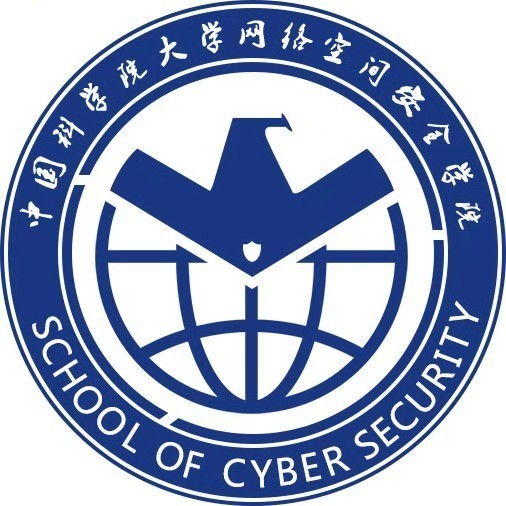
\includegraphics[width=0.25\textwidth]{images/title/Cyber.jpg}\\
	\vspace{1in}
}


\author{
	\hmwkAuthorName \\ 
	\hmwkAuthorStuID \\
	\hmwkAuthorInst \\
	\hmwkAuthorzhuanye \\
	\hmwkAuthorfangxiang
	}
\date{}

\renewcommand{\part}[1]{\textbf{\large Part \Alph{partCounter}}\stepcounter{partCounter}\\}


%
% 正文部分
%
\begin{document}


\maketitle


%\include{chapters/ch01}
%\include{chapters/ch02}
%\include{chapters/ch03}
%\include{chapters/ch04}
%\include{chapters/ch05}

\begin{homeworkProblem}
	请给出半监督学习常用的三种假设, 并分别列举出一种依据该假设所设计的半监督学习算法.

	\solution 半监督学习常用的三种假设和主要代表算法叙述如下:
	\begin{itemize}
		\item \textbf{平滑假设:} 如果\textbf{高密度空间}中两点$\boldsymbol{x}_1,\boldsymbol{x}_2$距离接近, 则对应的输出$y_1,y_2$也应该接近. 主要的代表算法是\textbf{生成式模型算法}.
		\item \textbf{聚类假设:} 如果两点在同一个簇, 那么它们很有可能属于同一个类. 主要的代表算法是\textbf{$\text{S}^3\text{VMs}$算法}.
		\item \textbf{流形假设:} \textbf{高维数据}大致会分布在一个低维的流形上, 并且邻近的样本拥有相似的输出. 主要的代表算法是\textbf{基于图的算法}.
	\end{itemize}
\end{homeworkProblem}

\begin{homeworkProblem}
	简述直推式和归纳式半监督学习算法的异同, 并分别例举出3种代表性算法.

	\solution 直推式和归纳式半监督学习的\textbf{相同点}是, 他们都使用少量有标注+大量无标注的数据集训练. 然而\textbf{不同点}在于: 直推式半监督算法关注模型在无标注数据集上的推理预测并且可以没有显式的学习函数$f$, 而归纳式半监督算法则关注于学习出一个显式函数$f$来对新的测试集进行推理. 直推式的代表性半监督算法有: $\text{TSVM}$算法、基于图的算法、半监督聚类. 归纳式的代表性半监督算法有: 自训练模型、多视图学习、生成式模型.
\end{homeworkProblem}


% 引用文献
%\bibliographystyle{unsrt}  % unsrt:根据引用顺序编号
%\bibliography{refs}


\end{document}
